\section{Results}
\label{results_section}

\subsection{Creating a representative dataset of questions}
\label{creating_dataset}

As described in \cref{dataset_creation}, we require a new and diverse dataset in order to run this data and answer the research question.

% We manually create a set of 4760 questions into 9 different categories, where each question 
We chose 9 different categories to ensure that the questions are varied and to study how the knowledge grounding of each model changes depending on the topic.
From those categories we manually wrote a set of 100 base questions and 411 objects, resulting in a total of 4760 initial queries.

\begin{enumerate}
	\item \textbf{Person} Historical people living from early antiquity to the present day from all around the globe. The questions have short, unambiguous answers, such as date of birth or most famous invention.
	\item \textbf{City} Cities from all over the globe. Questions may include population, founding date, notable landmarks, or geographical features.
	\item \textbf{Principle} Scientific principles, discovered from the 16th century forward. Questions about their discovery, use, and others.
	\item \textbf{Element} Elements from the periodic table. Questions may cover discovery, atomic number, chemical properties, or common uses.
	\item \textbf{Book} Literary works from various genres, time periods, and cultures. Questions may involve authors, publication dates, plot summaries, or literary significance.
	\item \textbf{Painting} Famous artworks from different art movements and periods. Questions may cover artists, creation dates, styles, or current locations.
	\item \textbf{Historical Event} Significant occurrences that shaped world history, from ancient times to the modern era. Questions may involve dates, key figures, causes, or their historical consequences.
	\item \textbf{Building} Notable structures from around the world, including ancient monuments, modern skyscrapers, and architectural wonders. Questions may cover location, architect, construction date, or architectural style.
	\item \textbf{Composition} Musical works from various genres and time periods. Questions may involve composers, premiere dates, musical style, or cultural significance.
\end{enumerate}

Each one of these categories has a number of questions that are assigned one of the objects, following and enhancing the question-building approach used by Yu et.\ al \cite{factual_recall}.

The total amount of these and composition of the 4760 questions can be found in \cref{category_amounts}.
The full set of questions can be found in the repository with the code used in this paper.

\begin{table}[ht]
	\centering
	\footnotesize
	\begin{tabular}{>{\bfseries}l r r r}
		\toprule
			\bfseries Category & \bfseries Base Questions & \bfseries Objects & \bfseries Total Questions \\
		\midrule
			Person           &  17 &  57 &  969 \\
			City             &  17 &  70 & 1190 \\
			Principle        &   5 &  37 &  185 \\
			Element          &  15 &  43 &  645 \\
			Book             &  11 &  49 &  539 \\
			Painting         &  12 &  44 &  528 \\
			Historical Event &   4 &  64 &  256 \\
			Building         &   9 &  22 &  198 \\
			Composition      &  10 &  25 &  250 \\
		\midrule
			Total            & 100 & 411 & 4760 \\
		\bottomrule \addlinespace[4pt]
	\end{tabular}
	\caption{The amount of base questions, objects, and the total amount of questions in each category on the final dataset after merging the base questions with the objects of each respective category.}
	\label{category_amounts}
\end{table}

\subsection{Framework Results}
\label{framework_results}

The results of running the queries created in \cref{creating_dataset} with added counterparametric context on each of the four models.

\Cref{total_table} shows the total type of answers for each one of the models; this information is plotted in \cref{total_plot}.

Additionally, \cref{cats_table} contains the information separated by question category.
How the category of each answer affects the amount of \Parametric{}, \Contextual{}, and \Other{} answers is discussed in the next sections.

\begin{table}[th]
	\centering
	\footnotesize
	\begin{tabular}{l r r r}
		\toprule
			\bfseries Model & \Pc{} & \Cc{} & \Oc{} \\
		\midrule
			\smallflan{}  & 248 & 4284 & 228 \\
			\bigflan{} & 242 & 4304 & 214 \\
		\midrule
			\smallllama{} & 745 & 3662 & 353 \\
			\bigllama{} & 1070 & 3303 & 387 \\
		\bottomrule \addlinespace[4pt]
	\end{tabular}
	\caption{Amount of answers of each category when running our dataset on each of the four models.}
	\label{total_table}
\end{table}

\begin{figure}[th]
	\centering
	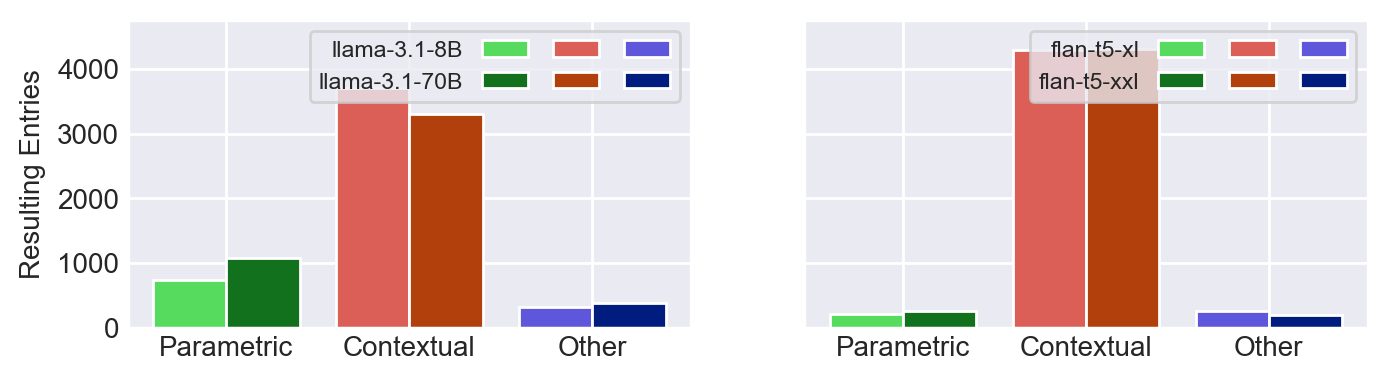
\includegraphics[width=\columnwidth]{both_amount.png}
	\caption{Amount of each answers of each category when running a context with counterparamteric information for Seq2Seq and Decoder-only models of different sizes.}
	\label{total_plot}
\end{figure}

\begin{table*}[t]
	\centering
	\footnotesize
	\begin{tabular}{>{\bfseries}l | r r r | r r r | r r r | r r r}
		\toprule
			& \multicolumn{3}{c|}{\smallflan{}} & \multicolumn{3}{c|}{\bigflan{}} & \multicolumn{3}{c|}{\texttt{llama-8B}} & \multicolumn{3}{c}{\texttt{llama-70B}}  \\
			& \Pc{} & \Cc{} & \Oc{} & \Pc{} & \Cc{} & \Oc{} & \Pc{} & \Cc{} & \Oc{} & \Pc{} & \Cc{} & \Oc{}  \\
		\midrule
			Person           &  32 &  900 & 37 &  23 &  890 & 56 &  40 &  833 & 96 & 209 & 614 & 146 \\
			City             & 120 & 1030 & 40 &  78 & 1093 & 19 & 117 & 1007 & 66 & 166 & 966 &  58 \\
			Principle        &  13 &  164 &  8 &   9 &  168 &  8 &  44 &  118 & 23 &  44 & 117 &  24 \\
			Element          &   6 &  637 &  2 & 102 &  515 & 28 & 218 &  385 & 42 & 275 & 347 &  23 \\
			Book             &  26 &  488 & 25 &  18 &  457 & 64 & 135 &  344 & 60 & 154 & 318 &  67 \\
			Painting         &  26 &  446 & 56 &   4 &  498 & 26 &  47 &  458 & 23 &  49 & 445 &  34 \\
			Historical Event &  11 &  217 & 28 &   1 &  254 &  1 &  81 &  154 & 21 & 117 & 118 &  21 \\
			Building         &  14 &  174 & 10 &   0 &  189 &  9 &  27 &  163 &  8 &  31 & 159 &   8 \\
			Composition      &   0 &  228 & 22 &   7 &  240 &  3 &  36 &  200 & 14 &  25 & 219 &   6 \\
		\bottomrule \addlinespace[4pt]
	\end{tabular}
	\caption{Results for running each one of the 10 categories separately.}
	\label{cats_table}
\end{table*}
